\section{A worked computation from first principles}\label{ch:worked}

Where Section~\ref{ch:classical} took the tilted route to large height, we return to the untilted route and follow one small computation with it at low height, from the theta series to a Thorin mass and a zero. Every value can be reproduced with \texttt{code/polya\_flint.py} (Section~\ref{app:code:eval}).

The parameters are those of Section~\ref{sec:ch4:trapezoid}, step $h=1/200$ and truncation $|u|\le3$, and the working precision is $240$ bits, about $72$ decimal digits, the default of the code. As there, $s$ is the displacement from $\frac12$: with $E=e^{sh}$ and $\Phi_j=\Phi(jh)$, the evaluator returns $\xi(\frac12+s)\approx P(E)+P(E^{-1})$ and $\xi'(\frac12+s)\approx Q(E)-Q(E^{-1})$, from which $\rho_\varepsilon(\theta)=\pi^{-1}\re(\xi'/\xi)(\frac12+\varepsilon+i\theta)$.

\paragraph{Step one: the kernel at a single point.} At $u=0$ the kernel \eqref{eq:ch2:Phi} is
\[
\Phi(0)=2\sum_{n\ge1}\big(2\pi^2n^4-3\pi n^2\big)e^{-\pi n^2}.
\]
The $n$th term is of order $n^4e^{-\pi n^2}$, and the terms with $n\ge8$ add up to less than $10^{-82}$, so seven terms already give more than eighty digits:
\[
\Phi(0)=0.89339380093424688817396933410941822644084873418965\ldots.
\]
The ball returned by the arithmetic has radius $3\times10^{-71}$.

\paragraph{Step two: the coefficients.} The truncation leaves $601$ nodes $u_j=jh$, $0\le j\le600$. The coefficients of $P$ are $\frac h2\Phi_0$ and $h\Phi_j$, $1\le j\le600$, and those of $Q$ are $h^2j\Phi_j$; the first is
\[
\tfrac h2\Phi(0)=0.00223348450233561722043492333527354556610\ldots.
\]
The coefficients decay doubly exponentially. By the asymptotic formula of Section~\ref{ch:clock}, $\Phi(2.7)\approx4\pi^2e^{12.15}\exp(-\pi e^{5.4})\approx6\times10^{-296}$, so the coefficients beyond $j\approx540$ are below $10^{-297}$.

\paragraph{Step three: $\xi(\frac12)$ as a trapezoid sum.} At $s=0$, $E=e^{sh}=1$, and $\xi(\frac12)=2P(1)$ is the trapezoid sum of the kernel:
\[
\xi(\tfrac12)=0.4971207781883141099127737396853977198072936095577\ldots,
\]
with ball radius $5\times10^{-71}$. \texttt{mpmath}'s evaluation from the definition, $\frac12z(z-1)\pi^{-z/2}\Gamma(z/2)\zeta(z)$ at $z=\frac12$ in thirty digit arithmetic, gives
\[
0.497120778188314109912773739685,
\]
agreeing to every digit. By the bound of Section~\ref{sec:ch4:trapezoid} the quadrature error is below $10^{-400}$, so the seventy digits are set by the working precision, not by the rule.

\paragraph{Step four: the Thorin density at the first ordinate.} At
\[
s=0.1+14.134725141734693790i,
\]
that is at resolution $\varepsilon=0.1$ and the first ordinate $\gamma_1$, the evaluator returns $\xi(\frac12+s)$ and $\xi'(\frac12+s)$, and
\[
\rho_{0.1}(\gamma_1)=\frac1\pi\re\frac{\xi'}{\xi}\Big(\frac12+s\Big)=3.18525309376337225967538\ldots.
\]
A single Cauchy kernel of width $0.1$ contributes exactly $1/(\pi\varepsilon)=3.18309886183791$ at its centre. By Proposition~\ref{prop:struct} the excess, $0.00215423$, is the sum of the contributions of every other zero, $\sum_{j\ne1}[P_{0.1}(\gamma_1-\gamma_j)+P_{0.1}(\gamma_1+\gamma_j)]$, plus the reflected kernel of $\gamma_1$ itself. The nearest neighbour, at distance $6.887$, contributes $6.7\times10^{-4}$, the reflected kernel $4\times10^{-5}$, and the many distant zeros, whose contributions decay like the inverse square of the distance, the remaining $1.4\times10^{-3}$. Figure~\ref{fig:ch5b:decomp} shows the same decomposition along the whole stretch between the first two zeros.

\begin{figure}[htbp]
\centering
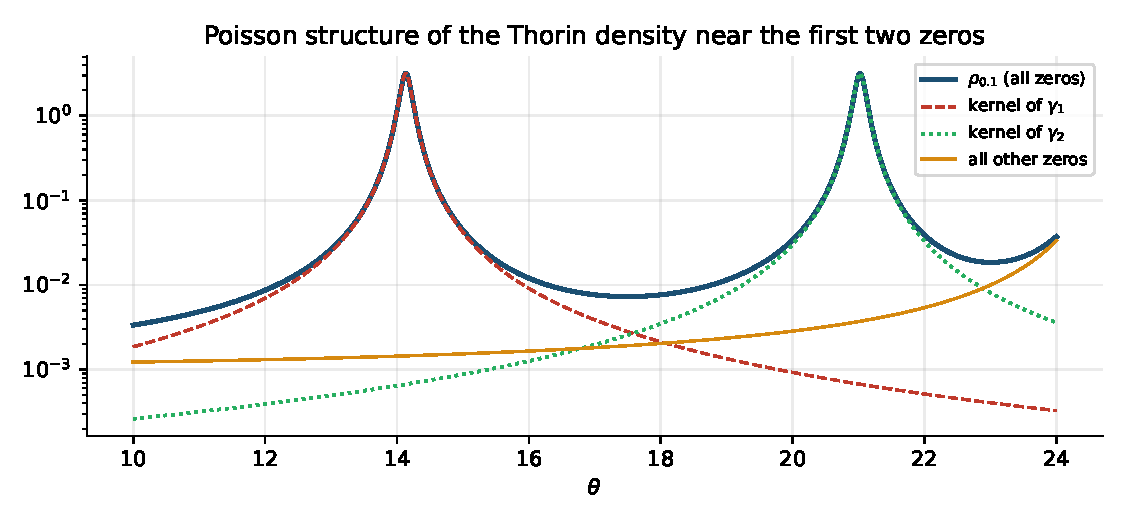
\includegraphics[width=0.85\textwidth]{fig/decomp.pdf}
\caption{The Thorin density $\rho_{0.1}$ near the first two zeros, split into the kernel of $\gamma_1$, the kernel of $\gamma_2$ and the rest, that is all other zeros and the reflected kernels at $-\gamma_j$, computed from the first $1700$ zeros without a tail correction.}
\label{fig:ch5b:decomp}
\end{figure}

Between zeros the density is small but strictly positive. At $\theta=17$, between $\gamma_1$ and $\gamma_2=21.022$,
\[
\rho_{0.1}(17)=0.0076857707896205949783\ldots,
\]
close to the minimum of $\rho_{0.1}$ between the two zeros (Figure~\ref{fig:ch5b:decomp}). Lagarias's criterion \cite{Lagarias} asks for this positivity at every $\theta$ and every resolution $\varepsilon>0$.

\paragraph{Step five: the Thorin mass up to height $20$.} The cumulative Thorin mass of Section~\ref{sec:ch4:height200} is $M_\varepsilon(\theta)=\mu_\varepsilon((0,\theta^2])=\pi^{-1}\arg\xi(\frac12+\varepsilon+i\theta)$, with the argument continued from the real axis. Stepping along the line $\frac12+0.1+i\theta$ from $\theta=0$ to $\theta=20$ in $1600$ steps of $\varepsilon/8=0.0125$, as in that section, and accumulating the arguments of the quotients $\xi(\frac12+s_{k+1})/\xi(\frac12+s_k)$, where $s_k=0.1+i\theta_k$ and $\theta_k=0.0125\,k$, gives
\[
\mu_{0.1}\big((0,400]\big)=M_{0.1}(20)=1.0509304\ldots,
\]
in $0.77$ seconds. There is exactly one zero below height $20$. By Proposition~\ref{prop:mass} the excess $0.0509$ over the count agrees to $O(\varepsilon^2)$ with the first order mass defect $-(\varepsilon/\pi)\Xi'(20)/\Xi(20)$ (Exercise~\ref{ex:ch5b:mass}): it is the mass carried across the edge $\theta=20$ by the Cauchy tails of the first zero and of the zeros above $20$, while what crosses $\theta=0$ is returned exactly by the reflected kernels. Adding $\tau_{0.1}(20)$, which is $\pi^{-1}$ times the change of $\arg\xi$ along the segment from $\frac12+0.1+20i$ to $\frac12+20i$, returns the integer $1$, as Proposition~\ref{prop:zerodensity} requires.

\paragraph{Step six: locating the first zero.} The ordinate $\gamma_1$ in step four was only a convenient point, and the density would have revealed it, up to the small shift caused by the other zeros, as the location of its first peak. To locate it from the P\'olya route alone, one evaluates $\Xi(\theta)=\xi(\frac12+i\theta)$ on a grid, finds the sign change in $(14.10,14.15)$, and refines by Newton's method with $\Xi'(\theta)=-\im\xi'(\frac12+i\theta)$; six iterations give $\gamma_1$ to forty digits. Section~\ref{sec:ch4:height200} refines all $79$ zeros below height $200$ in the same way, at $420$ bits.

